\subsection{Auswertung des Versuchs Elektronen im elektrischen Feld}
	
	Im Folgenden sind die während der Versuche aufgenommenen Daten
	und die aus diesen berechneten Ergebnisse tabellarisch und graphisch
	dargestellt. An entsprechender Stelle sind Erklärungen zu den 
	durchgeführten Rechnungen und Ergebnissen gegeben.
	Die für die Fehlerrechnung verwendeten Fehlergleichungen befinden 
	sich in \cref{sec:Fehlerrechnung} und sind mit römischen Ziffern nummeriert.
	

	\subsubsection{Ablenkung von Elektronen im elektrischen Feld}
	
		Die während den fünf Messdurchgängen aufgenommenen Werte für die
		Ablenk- und Beschleunigungsspannung sowie die Verschiebung sind in \cref{tab:Auswertung_Messdaten_I} zu finden.
		Die Fehler der Messwerte, wurden dabei mit der kleinsten Skaleneinteilung des 
		jeweiligen Messgerätes abgeschätzt.
				
			\begin{table}[!h]
	\centering
	\begin{tabular}{|c|c|c|c|}
		\hline
		Pos. Bild & Pos. Linse & Gegenstandsweite & Bildweite\\
		$x_{B}$ [\si{\centi\meter}] & $x_{L}$ [\si{\centi\meter}] & $g$ [\si{\centi\meter}] & $b$ [\si{\centi\meter}]\\
\hline\hline
		\num{89.6(1)} & \num{109.0(1)} & \num{20.0(1)} & \num{19.4(1)}\\
		\num{87.8(1)} & \num{104.0(1)} & \num{25.0(1)} & \num{16.2(1)}\\
		\num{84.4(1)} & \num{99.0(1)} & \num{30.0(1)} & \num{14.6(1)}\\
		\num{80.4(1)} & \num{94.0(1)} & \num{35.0(1)} & \num{13.6(1)}\\
		\num{76.0(1)} & \num{89.0(1)} & \num{40.0(1)} & \num{13.0(1)}\\
		\num{71.5(1)} & \num{84.0(1)} & \num{45.0(1)} & \num{12.5(1)}\\
		\num{66.9(1)} & \num{79.0(1)} & \num{50.0(1)} & \num{12.1(1)}\\
		\num{62.1(1)} & \num{74.0(1)} & \num{55.0(1)} & \num{11.9(1)}\\
		\num{57.2(1)} & \num{69.0(1)} & \num{60.0(1)} & \num{11.8(1)}\\
		\num{52.4(1)} & \num{64.0(1)} & \num{65.0(1)} & \num{11.6(1)}\\
		\hline
	\end{tabular}
	\caption{Gemessene Positionen des Bildes und der Linse und die daraus bestimmten 
		Bild- und Gegenstandsweiten für die Messreihe mit der bekannten Linse. Als Fehler wurde die kleinste Skaleneinteilung des
		verwendeten Millimetermaßes angenommen.  \label{tab:Auswertung_Messwerte_I}}
\end{table}
   
		
		In den Abbildungen \ref{fig:Auswertung_Messdaten_I_I}, \ref{fig:Auswertung_Messdaten_I_II},
		\ref{fig:Auswertung_Messdaten_I_III}, \ref{fig:Auswertung_Messdaten_I_IV} und
		\ref{fig:Auswertung_Messdaten_I_V} sind die 
		gemessenen Verschiebungen $D$ gegen die entsprechenden Ablenkspannungen $U_{d}$ aufgetragen.
		Die mittels lineare Ausgleichsrechnung mit dem Ansatz 
		\begin{empheq}{equation}
			D(U_{d}) = m \cdot U_{d} + b,
		\end{empheq} 
		unter Verwendung der Python Bibliothek \emph{SciPy} \cite{SciPy},
		berechneten Parameter $m_{i}, b_{i}$ sind in \cref{tab:Auswertung_Parameter_E} aufgelistet.
		
		\begin{table}[!h]
	\centering
	\begin{tabular}{|c|c|}
		\hline
		Steigung & y-Achsenabschnitt\\
		$m$ [\si{\meter\per\volt}] & $b$ [\si{\cm\meter}]\\
\hline\hline
		\num{0.173(2)} & \num{3.69(3)}\\
		\num{0.1082(8)} & \num{3.65(1)}\\
		\num{0.0930(9)} & \num{3.29(2)}\\
		\num{0.084(1)} & \num{3.72(2)}\\
		\num{0.066(1)} & \num{3.67(2)}\\
		\hline
	\end{tabular}
	\caption{Fit-Parameter der Daten aus den fünf Messreihen \label{tab:Auswertung_Parameter_E}}
\end{table}

		
		
		\begin{figure}[!h]
				\centering
				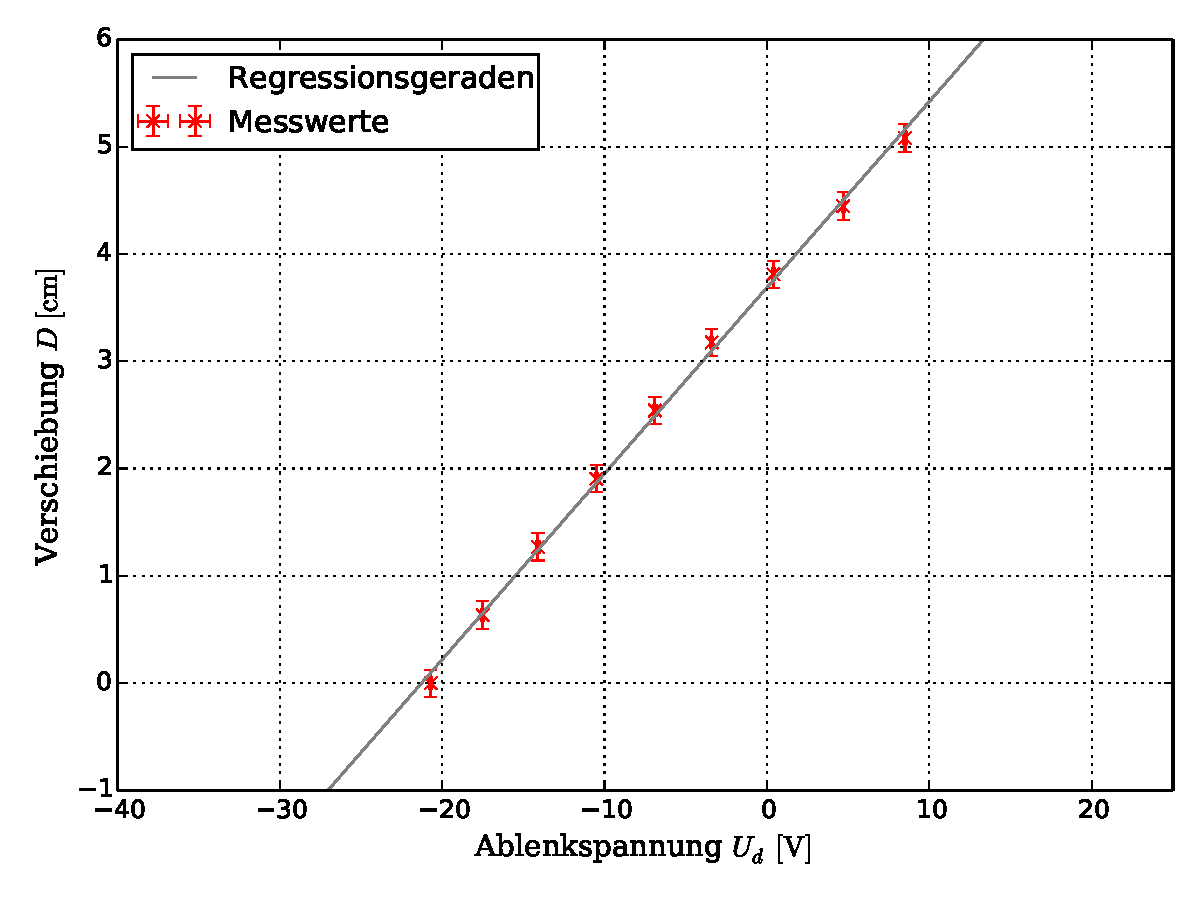
\includegraphics[scale=0.7]{Grafiken/EFeld_Messreihe_I.pdf}
				\caption{Grafische Darstellung der ersten Messreihe im E-Feld}
				\label{fig:Auswertung_Messdaten_I_I}
		\end{figure}
		
		\begin{figure}[!h]
		\centering
				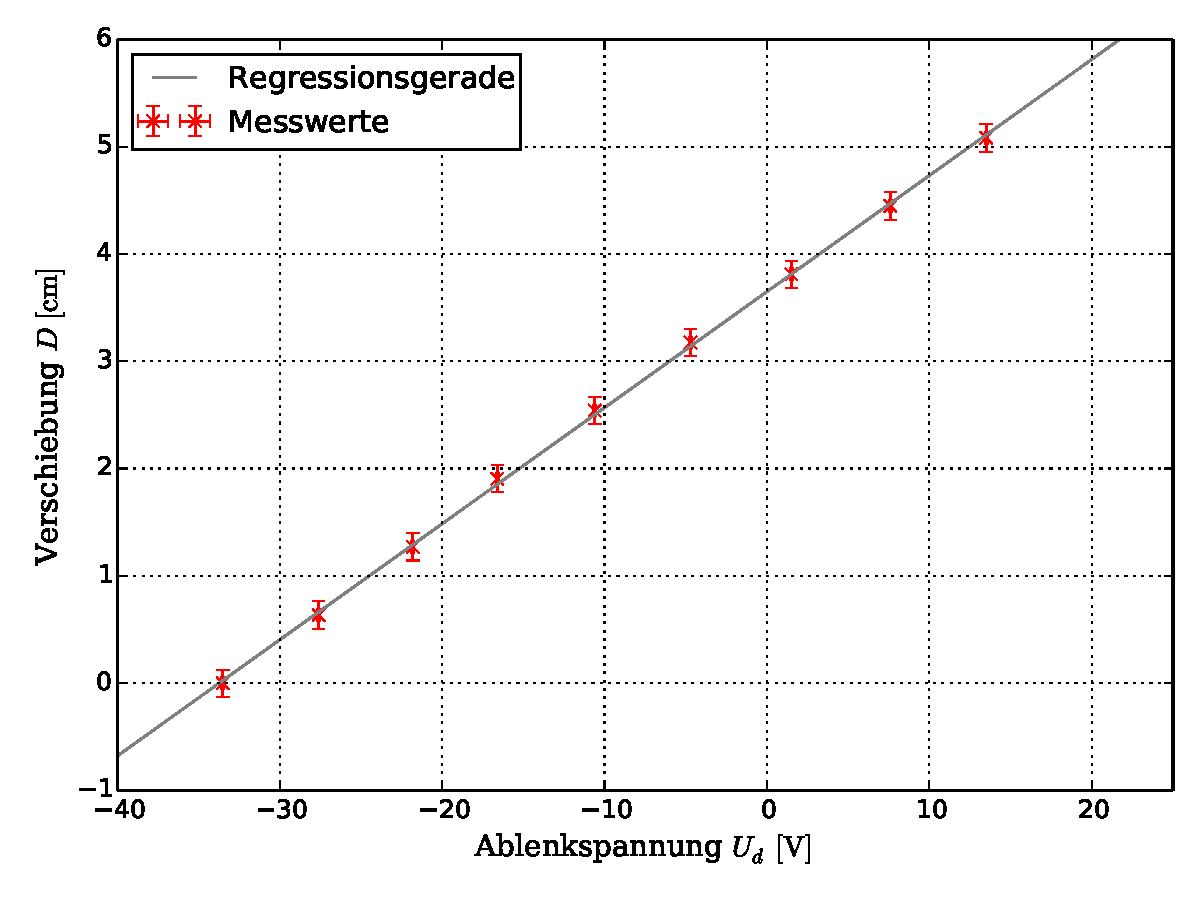
\includegraphics[scale=0.7]{Grafiken/EFeld_Messreihe_II.pdf}
				\caption{Grafische Darstellung der zweiten Messreihe im E-Feld}\label{fig:Auswertung_Messdaten_I_II}
		\end{figure}
		
		\begin{figure}[!h]
		\centering
				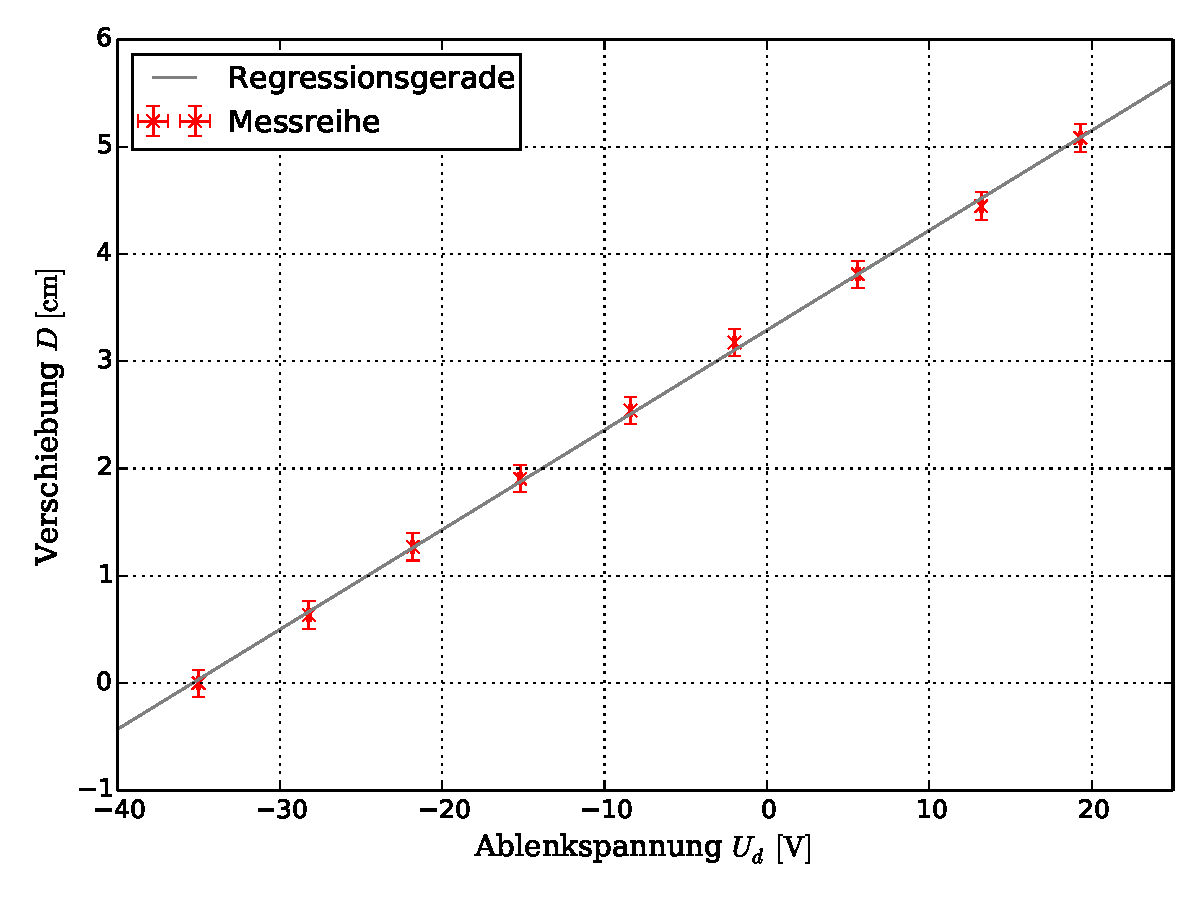
\includegraphics[scale=0.7]{Grafiken/EFeld_Messreihe_III.pdf}
				\caption{Grafische Darstellung der dritten Messreihe im E-Feld}\label{fig:Auswertung_Messdaten_I_III}
		\end{figure}
		
		\begin{figure}[!h]
		\centering
				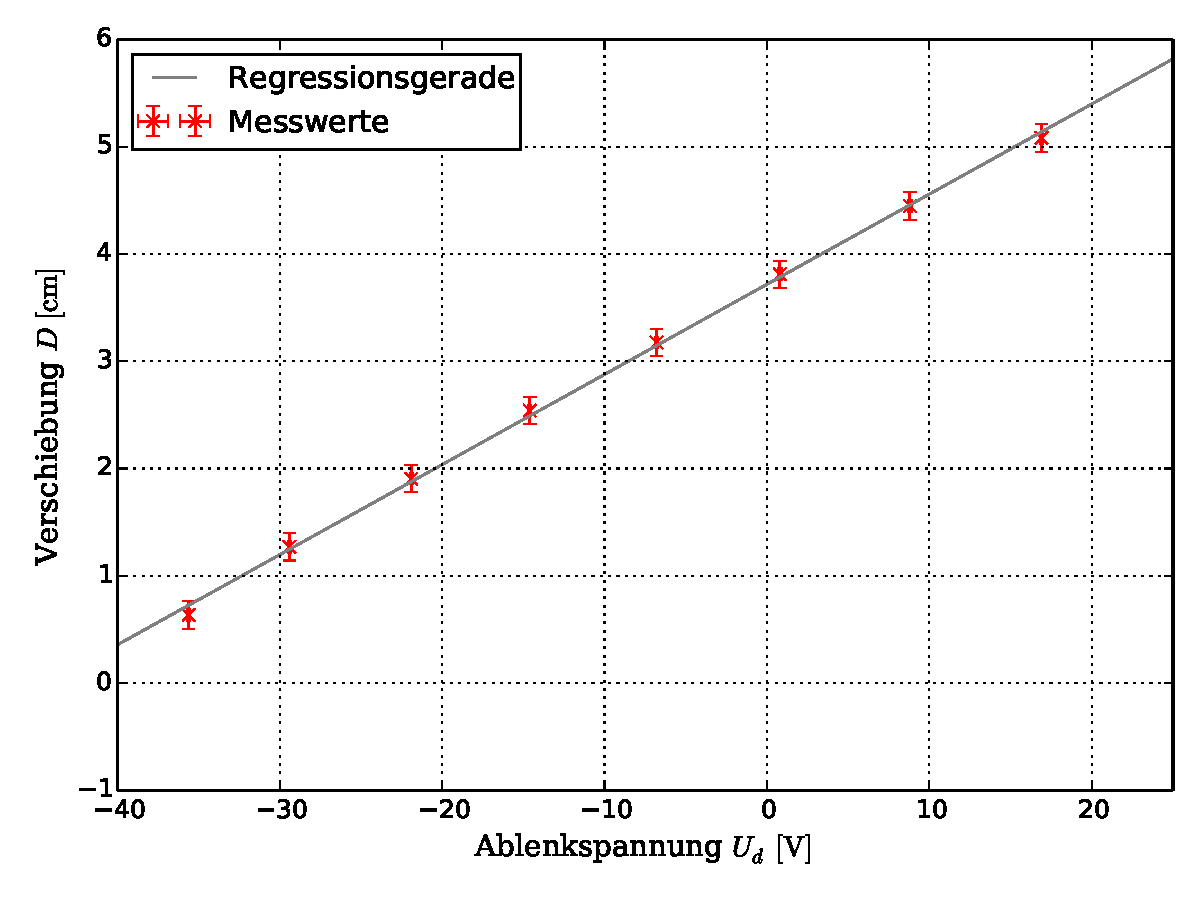
\includegraphics[scale=0.7]{Grafiken/EFeld_Messreihe_IV.pdf}
				\caption{Grafische Darstellung der vierten Messreihe im E-Feld}\label{fig:Auswertung_Messdaten_I_IV}
		\end{figure}
		
		\begin{figure}[!h]
		\centering
				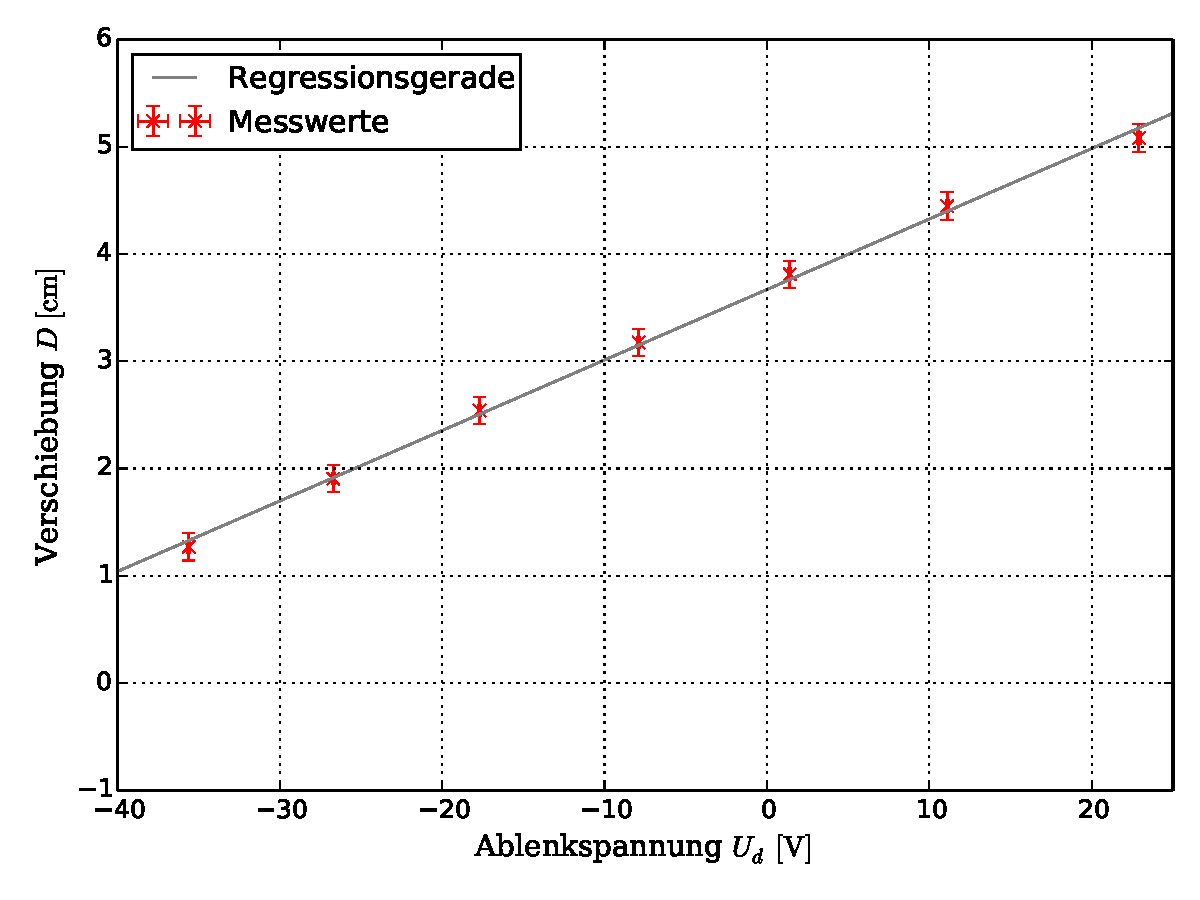
\includegraphics[scale=0.7]{Grafiken/EFeld_Messreihe_V.pdf}
				\caption{Grafische Darstellung der fünften Messreihe im E-Feld}\label{fig:Auswertung_Messdaten_I_V}
		\end{figure}
		
		Die Steigung dieser Graphen stellt die Empfindlichkeit $\frac{D}{U_{d}}$
		der Apparatur dar, die in \cref{fig:Auswertung_Messdaten_I_VI} gegen die reziproke 
		Beschleunigungsspannung aus \cref{tab:Auswertung_Messdaten_I} aufgetragen ist.
		
		\begin{figure}[!h]
		\centering
			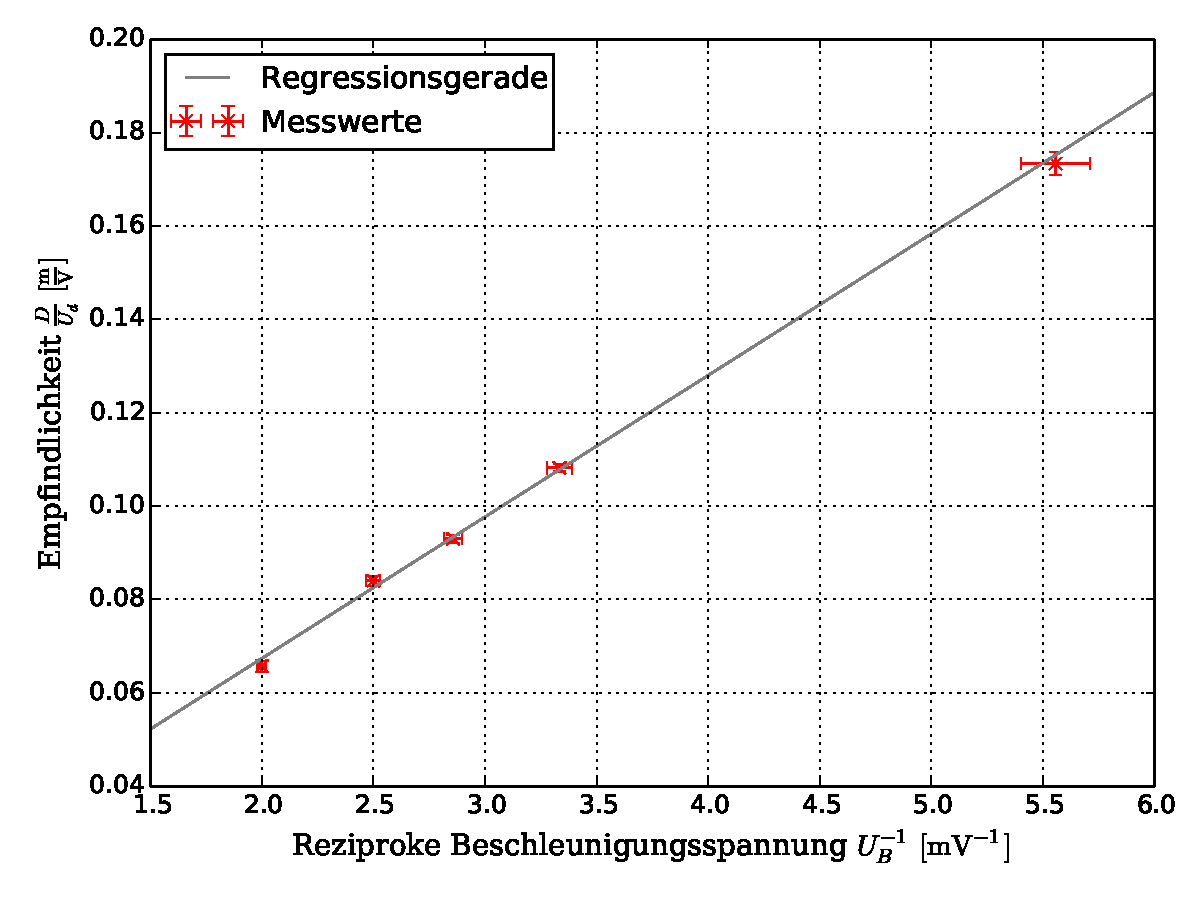
\includegraphics[scale=0.7]{Grafiken/EFeld_Messreihe_VI.pdf}
			\caption{Darstellung des Zusammenhangs von Empfindlichkeit Beschleunigungsspannung}\label{fig:Auswertung_Messdaten_I_VI}
		\end{figure}
		
		Die durch Regression mit dem  Ansatz
		\begin{empheq}{equation}
		\frac{D}{U_{d}}(U_{b}^{-1}) = \frac{\alpha}{U_{b}} + \beta ,
		\end{empheq} 		
		erhält man die Parameter
		\addtocounter{equation}{-1}
		\begin{subequations}
			\begin{empheq}{align} 
				\label{eq:Auswertung_Ergebnis_I}
				\alpha &= \SI{30.3(8)}{\centi\meter}\\ 
				\beta &= \SI{0.006(3)}{\centi\meter\per\volt}.
			\end{empheq}
		\end{subequations}
		
		Ein theoretischer Vergleichswert zu dem in \cref{fig:Auswertung_Messdaten_I_VI} 
		dargestellten Zusammenhang erhält man mittels \cref{eq:Theorie_D} und den
		Angaben im Bauplan \cite{V501} der Kathodenstrahlröhre zu den Maßen
		$L = \SI{14.5}{\centi\meter}$, $p = \SI{1.9}{\centi\meter}$ und $d = \SI{0.38}{\centi\meter}$.
		
		Aus den genannten Größen berechnet sich die theoretische Steigung der 
		Geraden in \cref{fig:Auswertung_Messdaten_I_VI} zu
		\begin{empheq}{equation}
			\label{eq:Auswertung_Ergebnis_I_theo} 
			\alpha_{theo} = \SI{36.25}{\centi\meter}.
		\end{empheq}	
%		\begin{figure}[!h]
%			\centering
%			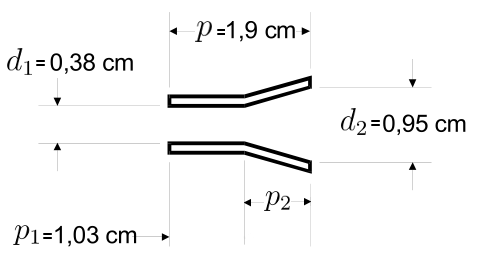
\includegraphics[scale=0.7]{Grafiken/Bauplan.PNG}
%			\caption{Bauplan der x-Ablenkung, bearbeitet aus \cite{V501}}\label{fig:Auswertung_Bauplan}
%		\end{figure}
		
	\subsubsection{Stehende Sinuswellen am Oszilloskop}

		Die zur Erzeugung eingestellten Sägezahn-Frequenzen $f_{sz}$ sind
		mit den Verhältnissen $n$ und der aus diesen berechneten Sinus-Frequenz
		$f_{sin}$ in \cref{tab:Auswertung_Oszilloskop} eingetragen.
		
		\begin{table}[!h]
	\centering
	\begin{tabular}{|c|c|c|}
		\hline
		Sägezahn-Frequenz & Verhältnis & Sinus-Frequenz\\
		$f_{sz}$ [\si{\hertz}] & $n$ & $f_{sin}$ [\si{\hertz}]\\
\hline\hline
		\num{19.96(1)} & \num{4} & \num{79.84(4)}\\
		\num{39.94(1)} & \num{2} & \num{79.88(2)}\\
		\num{79.84(1)} & \num{1} & \num{79.84(1)}\\
		\num{159.68(1)} & \num{0.5} & \num{79.84(1)}\\
		\hline
	\end{tabular}
	\caption{Frequenzen $f_{sz}$ und $f_{sin}$ für stehende Wellen \label{tab:Auswertung_Oszilloskop}}
\end{table}
 
		
		Der Mittelwert der berechneten Frequenzen ergibt sich zu
		\begin{empheq}{equation}
			\label{eq:Auswertung_Frequenz} 
			f = \SI{79.85(1)}{\centi\meter}.
		\end{empheq} 
		Der Fehler wurde dabei Mittels gaußscher Fehlerfortpflanzung berechnet, da der so erhaltene
		Fehler größer als die Abweichung vom Mittelwert ist.
		
\subsection{Auswertung des Versuchs Elektronen im magnetischen Feld}

	\subsubsection{Ablenkung von Elektronen im magnetischen Feld}
	
		Die in den vier Messreihen aufgenommenen Werte für Ablenkstrom $I_{d}$,
		die daraus resultierende Verschiebung $D$ und die jeweilige 
		Beschleunigungsspannung $U_{b}$ befinden sich in 
		\cref{tab:Auswertung_Messdaten_II} und das von dem Strom $I_{d}$ 
		erzeugte und mit \cref{eq:Theorie_Magnetfeld} berechnete Magnetfeld $B_{d}$ in 
		\cref{tab:Auswertung_Messdaten_II_B}. Auch hier wurde der Fehler des Stroms 
		mit der kleinsten Skaleneinheit des Messgerätes abgeschätzt.
		
		\begin{table}[!h]
	\centering
	\begin{tabular}{|c|c|c|c|c||c|}
		\hline
		Messreihe & 1 & 2 & 3 & 4 & Verschiebung\\
		Nr. &$$ & $$ & $$ & $$ & $D$ [\si{\centi\meter}]\\
\hline
\multirow{7}{1.75cm}{Ablenk-\\ strom\\$\quad\!I_{d}$\ [\si{\ampere}]}		&\num{0.00(1)} & \num{0.00(1)} & \num{0.00(1)} & \num{0.00(1)} & \num{0.0(1)}\\
		&\num{0.32(1)} & \num{0.36(1)} & \num{0.38(1)} & \num{0.38(1)} & \num{0.6(1)}\\
		&\num{0.68(1)} & \num{0.74(1)} & \num{0.82(1)} & \num{0.84(1)} & \num{1.3(1)}\\
		&\num{1.00(1)} & \num{1.10(1)} & \num{1.20(1)} & \num{1.15(1)} & \num{1.9(1)}\\
		&\num{1.30(1)} & \num{1.45(1)} & \num{1.60(1)} & \num{1.60(1)} & \num{2.5(1)}\\
		&\num{1.65(1)} & \num{1.80(1)} & \num{1.95(1)} & \num{2.00(1)} & \num{3.2(1)}\\
		&\num{2.00(1)} & \num{2.20(1)} & - & - & \num{3.8(1)}\\
		&\num{2.25(1)} & - & - & - & \num{4.4(1)}\\ \hline
\multirow{3}{1.75cm}{Beschl.\\Spannung\\$\quad\!U_{b}$\ [\si{\volt}]}	& & & & & \\
				 							   & \num{250(5)}   &   \num{300(5)}  & \num{350(5)}  & \num{400(5)} &  
				 							   \\ 
				 							   &&&&&\\\hline
		
		
		\hline
	\end{tabular}
	\caption{Messdaten zur Bestimmung des Zusammenhangs zwischen $I_d$ und $D$ \label{tab:Auswertung_Messdaten_II}}
\end{table}

		\begin{table}[!h]
	\centering
	\begin{adjustbox}{width=1\textwidth, center}
	\begin{tabular}{|c|c|c|c|c||c|}
		\hline
	Messreihe & 1 & 2 & 3 & 4 & Verschiebung\\
	Nr.	&$$ & $$ & $$ & $$ & $D$ [\si{\centi\meter}]\\
\hline
	\multirow{8}{1.75cm}{Ablenk-\\ B-Feld\\$\; B_{d}$\ [\si{\milli\tesla}]}	&\num{0.0000(6)} & \num{0.0000(6)} & \num{0.0000(6)} & \num{0.0000(6)} & \num{0.0(1)}\\
		&\num{0.0204(6)} & \num{0.0230(6)} & \num{0.0242(6)} & \num{0.0242(6)} & \num{0.6(1)}\\
		&\num{0.0434(6)} & \num{0.0472(6)} & \num{0.0523(6)} & \num{0.0536(6)} & \num{1.3(1)}\\
		&\num{0.0638(6)} & \num{0.0701(6)} & \num{0.0765(6)} & \num{0.0733(6)} & \num{1.9(1)}\\
		&\num{0.0829(6)} & \num{0.0925(6)} & \num{0.1020(6)} & \num{0.1020(6)} & \num{2.5(1)}\\
		&\num{0.1052(6)} & \num{0.1148(6)} & \num{0.1244(6)} & \num{0.1275(6)} & \num{3.2(1)}\\
		&\num{0.1275(6)} & \num{0.1403(6)} & - & - & \num{3.8(1)}\\
		&\num{0.1435(6)} & -& - & - & \num{4.4(1)}\\ \hline
		\multirow{3}{1.75cm}{Beschl.\\Spannung\\$\quad\!U_{b}$\ [\si{\volt}]}	& & & & & \\
		& \num{250(5)}   &   \num{300(5)}  & \num{350(5)}  & \num{400(5)} &  \\ 
	    &	&	&	&	&	\\
		
		
		
		
		\hline
	\end{tabular}
	\end{adjustbox}
	\caption{Messdaten zur Bestimmung des Zusammenhangs zwischen $B_d$ und $D$ \label{tab:Auswertung_Messdaten_II_B}}
\end{table}

		
		In den Abbildungen \ref{fig:Auswertung_Messdaten_II_I}, \ref{fig:Auswertung_Messdaten_II_II}
		\ref{fig:Auswertung_Messdaten_II_III} und \ref{fig:Auswertung_Messdaten_II_IV}
		ist der Quotient $D'=\frac{D}{D^{2} + L^{2}}$ mit der Länge der Kathodenstrahlröhre 
		$L = \SI{17.5}{\centi\meter}$ und der gemessenen Verschiebung $D$ gegen die
		jeweilige Magnetfeldstärke $B_{d}$ aufgetragen.
		Die Regressionsparameter der linearen Regression mit dem Ansatz
		\begin{empheq}{equation}
			D'(B_{d}) = \gamma \cdot B_{d} + \delta,
		\end{empheq} 
		befinden sich in \cref{tab:Auswertung_Parameter_B}.
		
		\begin{table}[!h]
	\centering
	\begin{tabular}{|c|c|}
		\hline
		Steigung & y-Achsenabschnitt\\
		$\gamma$ [\si{\meter\per\volt}] & $\delta$ [\si{\per\meter}]\\
\hline\hline
		\num{94(1)} & \num{0.010(9)}\\
		\num{85(1)} & \num{0.01(1)}\\
		\num{80.0(8)} & \num{0.002(6)}\\
		\num{79(2)} & \num{0.01(1)}\\
		\hline
	\end{tabular}
	\caption{Fit-Parameter der Daten aus den vier Messreihen \label{tab:Auswertung_Parameter_B}}
\end{table}

		
		\begin{figure}[!h]
		\centering
				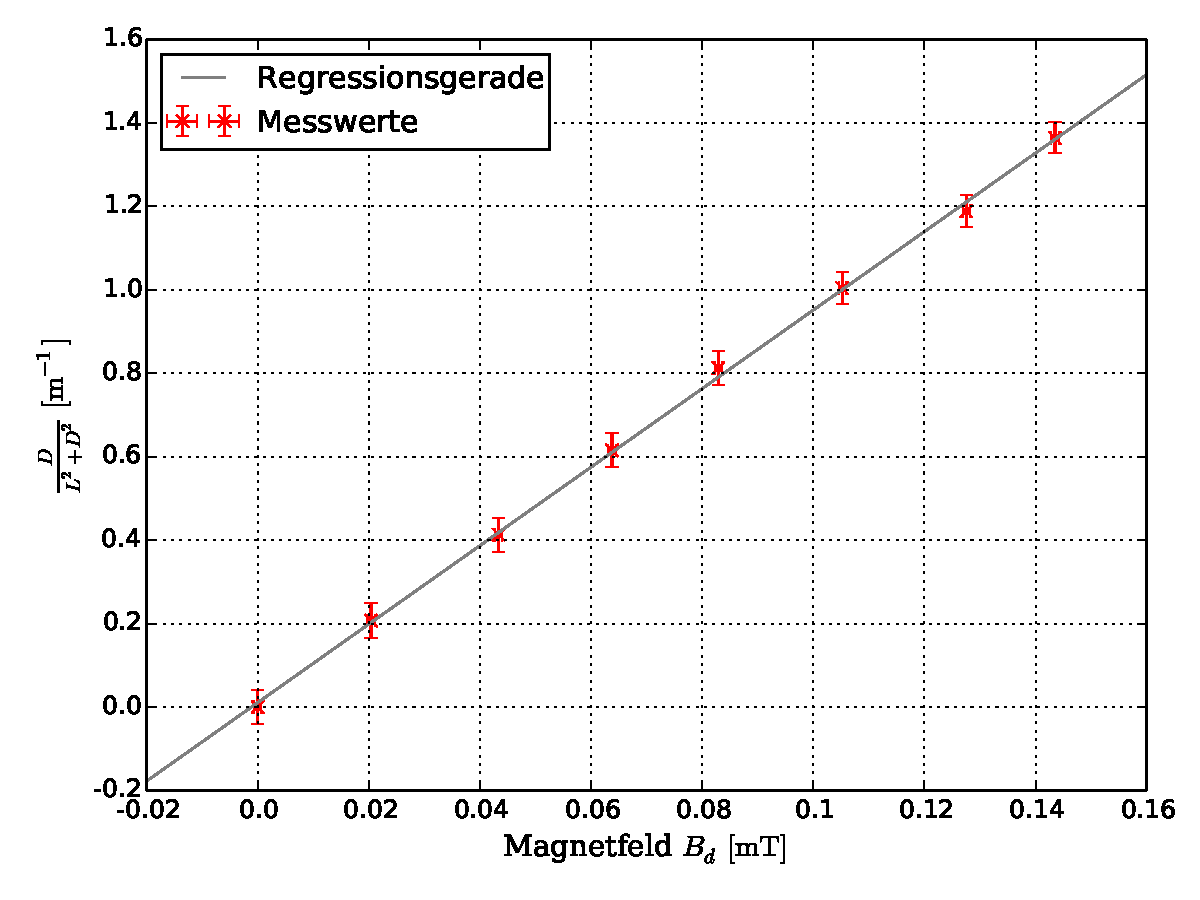
\includegraphics[scale=0.7]{Grafiken/BFeld_Messreihe_I.pdf}
				\caption{Grafische Darstellung der ersten Messreihe im B-Feld}\label{fig:Auswertung_Messdaten_II_I}
		\end{figure}
		
		\begin{figure}[!h]
			\centering
			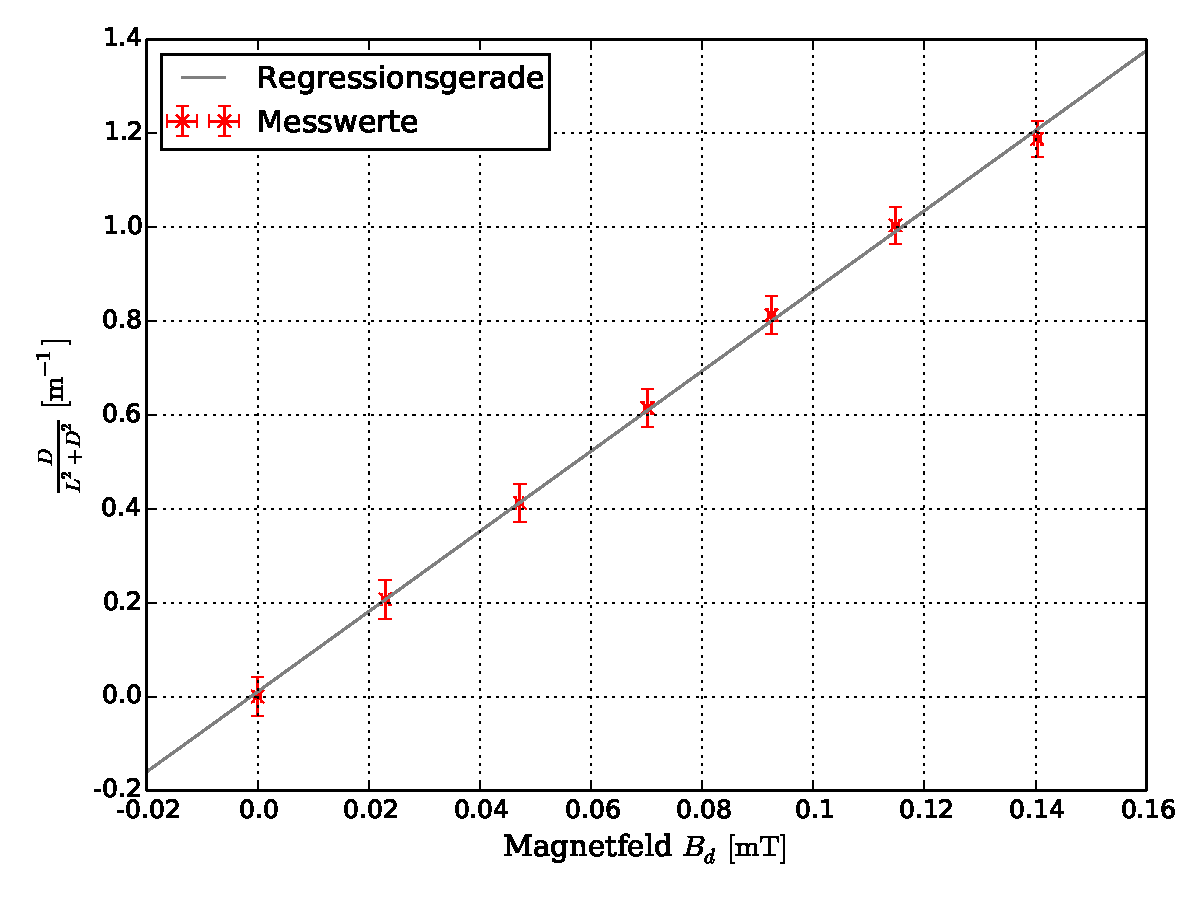
\includegraphics[scale=0.7]{Grafiken/BFeld_Messreihe_II.pdf}
			\caption{Grafische Darstellung der zweiten Messreihe im B-Feld}\label{fig:Auswertung_Messdaten_II_II}
		\end{figure}
		\begin{figure}[!h]
		\centering
			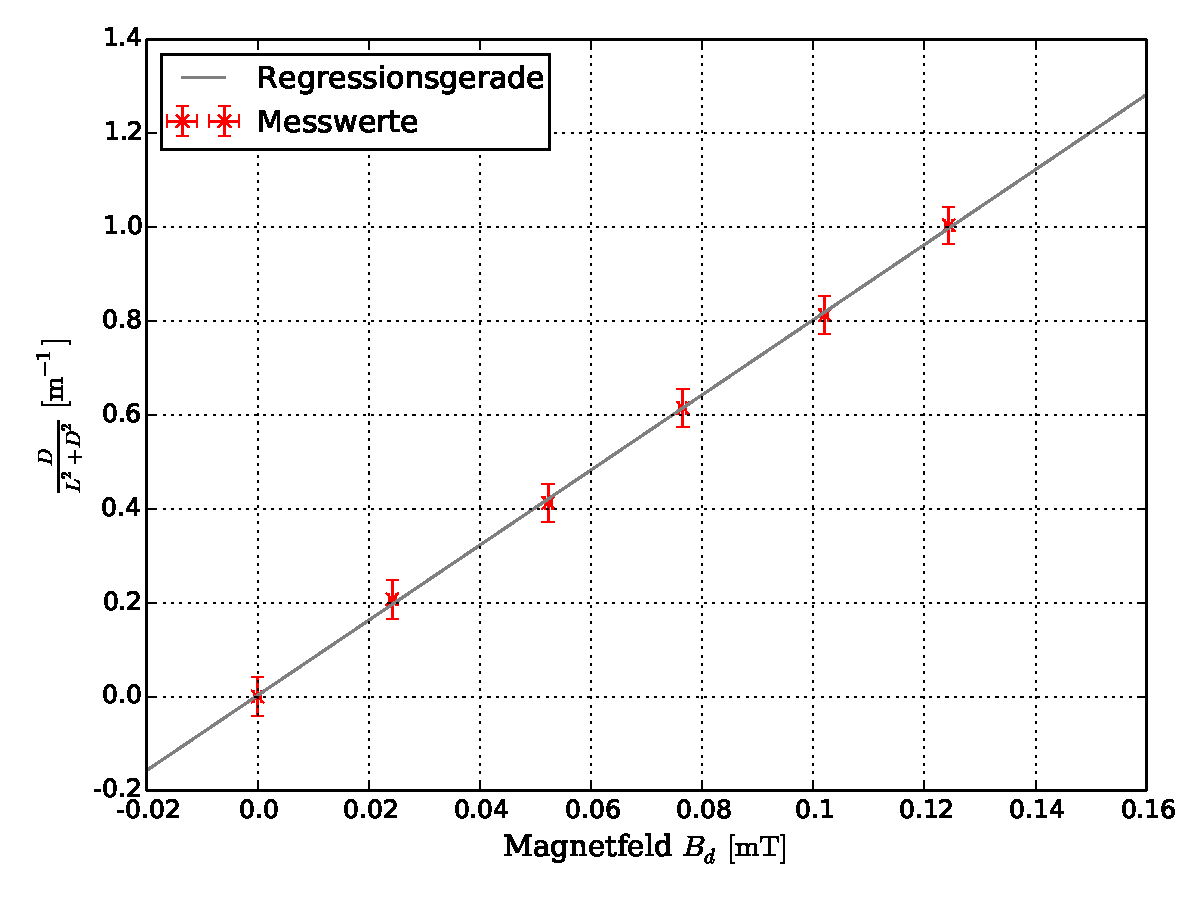
\includegraphics[scale=0.7]{Grafiken/BFeld_Messreihe_III.pdf}
			\caption{Grafische Darstellung der dritten Messreihe im B-Feld}\label{fig:Auswertung_Messdaten_II_III}
		\end{figure}
		\begin{figure}[!h]
		\centering
			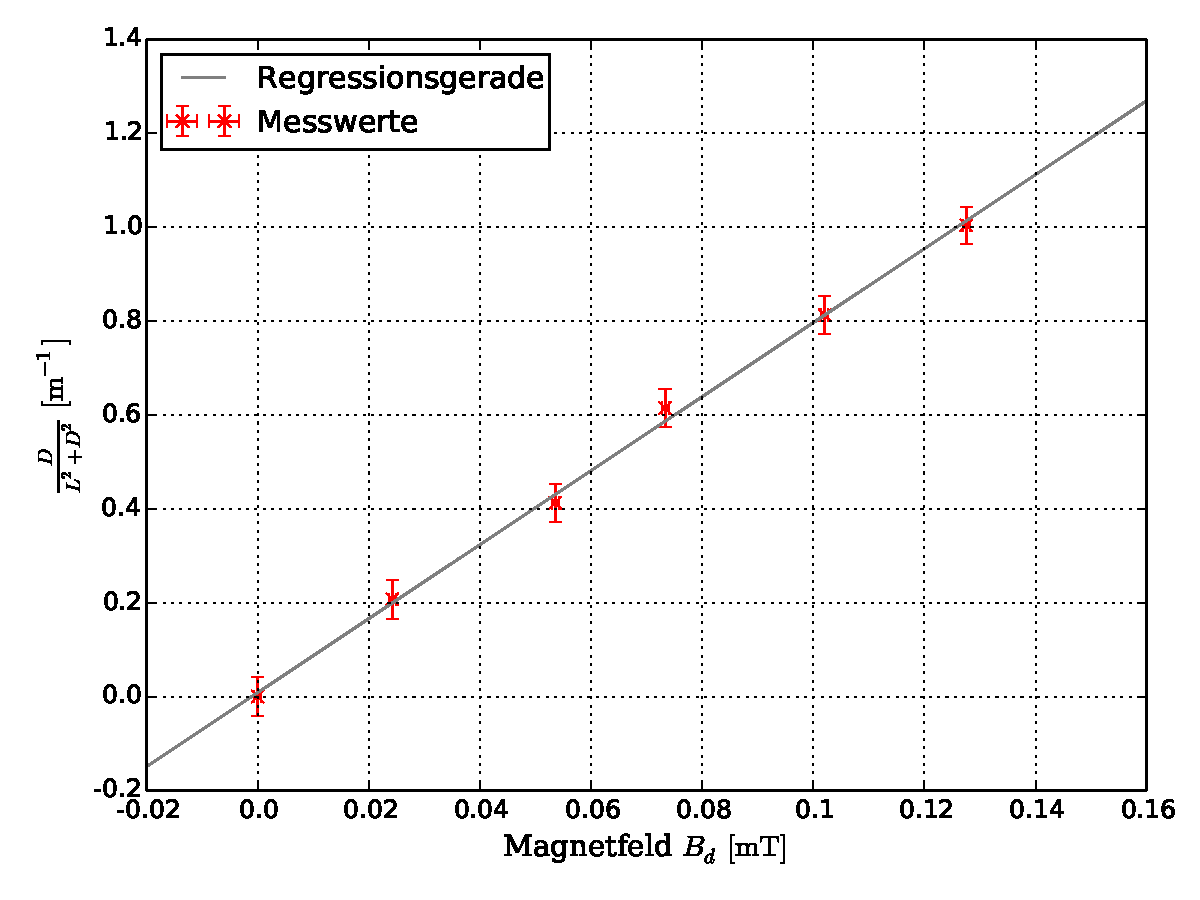
\includegraphics[scale=0.7]{Grafiken/BFeld_Messreihe_IV.pdf}
			\caption{Grafische Darstellung der vierten Messreihe im B-Feld}\label{fig:Auswertung_Messdaten_II_IV}
		\end{figure}

		Die ebenfalls in \cref{tab:Auswertung_Parameter_B} angegebene spezifische Ladung des Elektrons lässt sich nun unter Umformung von \cref{eq:Theorie_Qspez} zu 
		\begin{empheq}{equation} 
			\frac{e_{0}}{m_{e}} = 8 \cdot \gamma^{2} \cdot U_{b}  
		\end{empheq}	
		aus der Steigung $\gamma$ der Regressionsgeraden berechnen.
		
		Der Mittelwert der drei Messwerte mit der geringsten Abweichung vom Literaturwert
		ergeben im Mittel
		\begin{empheq}{equation}
			\label{eq:Auswertung_Qspez} 
			\frac{e_{0}}{m_{e}} = \SI{1.77(3)e11}{\coulomb\per\kg}.
		\end{empheq}
		Auch der Fehler dieses Wertes wurde mit Hilfe der gaußschen Fehlerfortpflanzung bestimmt, 
		da dieser Fehler der im Vergleich zur Abweichung vom Mittelwert größer ist. 
\newpage		
	\subsubsection{Bestimmung der Intensität des Erdmagnetfeldes}
	
		Für den Ausgleich der von dem Erdmagnetfeld verursachten Verschiebung wurde die Stromstärke
 		\begin{empheq}{equation}
 			I_{hor} = \SI{0.28(1)}{\ampere}
 		\end{empheq}
		an die Helmholtz-Spule angelegt. Mit \cref{eq:Theorie_Magnetfeld} 
		ergibt sich damit der Betrag des Erdmagnetfelds zu 
 		\begin{empheq}{equation}
 			B_{hor} = \SI{0.0179(6)}{\milli\tesla}.
 		\end{empheq}
 		
 		Die totale Intensität des Erdmagnetfeldes erhält ist mit dem Inklinationswinkel 
 		$\varphi = \SI{70}{\degree}$ zu
 		\begin{empheq}{equation}
 			\label{eq:Auswertung_Btotal}
 			B_{total} = \frac{B_{hor}}{\Cos{\varphi}} = \SI{52(2)}{\micro\tesla}.
 		\end{empheq}
 		bestimmbar.
